% https://tex.stackexchange.com/questions/370121/how-to-label-a-segment-in-tkz-euclide
% https://tex.stackexchange.com/questions/220503/how-to-shift-curly-brackets

\documentclass[12pt]{article}
\usepackage[utf8]{inputenc}
\usepackage{tikz, pgfplots, tkz-euclide}
\usetikzlibrary{positioning, decorations.text}

\usetikzlibrary{decorations.pathreplacing}

\begin{document}

\section{Kepler's Second Law Derivation}

\subsection{Review of Calculus}

\subsubsection{Limits and Derivatives}
\begin{sloppypar}
  Limits describe the behavior of a function near a point. For example, $\displaystyle{\lim_{x \to 2} x + 4 = 6}$
  since $2 + 4 = 6$.
  Special limits like
  $$\lim_{h \to 0} \frac{f(x+h)-f(x)}{h}$$
  represent the derivative, or instantaneous slope, of a function at a point.
  Similarly, you may take for granted that an expression like
  $$\lim_{t \to 0} \frac{\Delta x}{\Delta t} = \frac{dx}{dt} .$$
\end{sloppypar}

\subsubsection{Integration}
The power rule of integration for any function $x$ is as follows:
$$\int_{}^{} x^n \,dx = \frac{x^{n+1}}{n+1} + C .$$

\subsection{Definition}
A line joining a planet and the Sun sweeps out equal areas during equal intervals of time.

\subsection{Derivation}
For this line to sweep out equal area during equal time,
the rate at which the area changes, $\frac{dA}{dt}$ must stay constant.
One small slice of the area of a planet's elliptical orbit may be represented as
a triangle

$$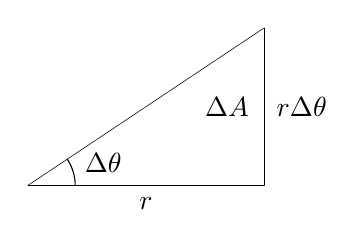
\begin{tikzpicture}

    \tkzDefPoint(0,0){A}
    \tkzDefPoint(3,2){B}
    \tkzDefPoint(3,0){C}

    \tkzDrawSegments(A,B B,C C,A)

    \tkzLabelSegment[below=1pt](C,A){$r$}
    \tkzLabelSegment[right=1pt](B,C){$r \Delta \theta$}

    \tkzMarkAngle[size=0.60cm](C,A,B)
    \tkzLabelAngle(C,A,B){$\Delta \theta$}

    \tkzLabelSegment[left=2pt](B,C){$\Delta A$}

  \end{tikzpicture}$$

with base $r$, height $r \Delta \theta$, and area $\Delta A$ (recall that arc length is $r \Delta \theta$).\\
Recall the equation for the area of a triangle,
$$A = \frac{1}{2}bh .$$
Substituing the givens from our slice above, we get
$$\Delta A = \frac{1}{2} (r) (r \Delta \theta) .$$
Divide both sides by $\Delta t$
$$\frac{\Delta A}{\Delta t} = \frac{1}{2} (r) (r \frac{\Delta \theta}{\Delta t}) .$$
Take the limit of boths sides as $\Delta t \to 0$ to find an ``infinitely'' small change of area over
an ``infinitely'' small change of time (keep in mind that $r$ is constant for our slice and that area $A$ is a function of time).
$$\lim_{\Delta t \to 0} (\frac{\Delta A}{\Delta t}) = \lim_{\Delta t \to 0} (\frac{1}{2} (r) (r \frac{\Delta \theta}{\Delta t})) ,$$
which simplifies to
$$\frac{dA}{dt} = \frac{1}{2} (r) (r \frac{d\theta}{dt})$$
and further simplies to
$$\frac{dA}{dt} = \frac{1}{2} r v_t .$$
Recall that angular momentum is
$$L = mrv_t$$
and is a conserved quantity. Substiting L into our area gets
$$\frac{dA}{dt} = \frac{L}{2m} .$$
We can then rearrange and solve the differential equation
$$\int_{}^{} \,dA = \int_{}^{} \frac{L}{2m} \,dt ,$$
which shows us that
$$A = \frac{L}{2m} T .$$
This shows us a directly proportional relationship between the area $A$ and time $T$.
\end{document}
